\section{Benchmark Results for the Onset of Rising Tone Chorus}
\label{sec:code}
We now conduct several simulations and apply our method to explore the onset of the whistler-mode chorus.
%(useless) We only consider the parallel propagated chorus wave, which is consistent with our approximation. 
% redundent The chorus wave has a pure right-handed polarization, thus $a(s_i,t)$ and $j_{p}$ in Eqs.~(\ref{eq.Wave}) and (\ref{eq.Wave1st}) can be expressed in a complex scalar, i.e., $a = a_x + \imath a_y$.
% useless The chorus is excited by left propagated resonant electrons, thus the wave propagates toward the right pole along the magnetic field line as a result.
%Based on our simulation model introduced previously, we first show some benchmark results, including linear whistler-mode instability to non-linear chorus wave generation and amplification. 
The unstable whistler wave is generally arising from the electron temperature anisotropy instability \cite{kennel1966a,kennel1966b}, and the growth rate can be obtained from the linear resonance condition near $\Omega \approx 0$.
%\begin{equation}
%    \begin{aligned}
%        D\left(\omega_l, k_l ; s\right) & =k_l^2(s)-\omega_l^2-\frac{\omega_p^2(s) \omega_l}{\omega_{c e}(s)-\omega_l} \\
%        & -\left.\imath 2 \pi^2 \frac{\omega_{c e}(s) \omega_{h 0}^2}{k_l(s)} \int_{-\Pi}^{\infty} d J(J+\Pi) \frac{\partial f_0}{\partial \Omega}\right|_{\Omega=0}=0
%        \end{aligned}
%\end{equation}

In our simulation, the energetic electron distribution is bi-Maxwellian at the magnetic equator. 
The equilibrium distribution within the $i^{th}$ cell remains the same form as the distribution in the phase space $(s_i, p_\|, \phi, \varphi)$, i.e.,
\begin{equation}
    \begin{aligned}
        & f_{i 0}(\xi, \Omega, \vartheta, J) =\frac{\omega_{c e 0}}{(2 \pi)^{3 / 2} v_{t h \perp 0}^2 v_{t h \| 0}} \frac{1}{1-\beta} \cdot \exp \left(-\frac{k_l^2(\Omega+\Pi_i)^2}{2 v_{t h \| 0}^2}\right) \\
        &\cdot\left(\exp \left(-\frac{(J+\Omega+\Pi_i) \omega_{c e 0}}{v_{t h \perp 0}^2}\right)-\exp \left(-\frac{(J+\Omega+\Pi_i) \omega_{c e 0}}{\beta v_{t h \perp 0}^2}\right)\right)~,
        \end{aligned}
\end{equation}
where $\beta$ is the depth of the loss cone, the subscript $0$ denotes the magnetic equator.


As a realistic model for the magnetosphere, the magnetic field can be approximated as a dipole field, and the major component of the background magnetic field near the equator can be approximately represented by a parabolic function \cite{tao_numerical_2014}
\begin{equation}
    B(\lambda) = B_0(1+ R_a \lambda ^2)~,
\end{equation}
where $R_a$ is the inhomogeneity ratio of the magnetic field, $B_0$ is the magnetic field strength at the equator, and $\lambda$ is the magnetic latitude. The distance alone the magnetic field line $s$ satisfies $s = L R_E \lambda$.
The background electron density is found to fit a power law form \cite{denton2004},
\begin{equation}
    n(\lambda) = n_0 (1+R_b \lambda^2)~
\end{equation}
where $R_b$ is a fitting parameter in an order of one.

\subsection{Simulation configuration}
In conventional PIC simulations, the inhomogeneity ratio $R_a$ was often enlarged by one or two order of magnitudes to reduce the simulation cost.
While, one of the benefits of our numerical scheme is that we can apply the realistic parameters of the Earth dipole field.
The basic parameters of our simulation are given in Tab. (\ref{tab.parameters}).
\begin{table}\label{tab.parameters}
    \centering
    \caption{Magnetic field and plasma parameters used in the simulation.\newline}
    \begin{tabular}{lc}
    \hline
     L-shell of the magnetic field line  & 5 \\
     Magnetic field inhomogeneity ratio $R_a$ &  4.5 \\
     Background cold plasma density inhomogeneity ratio $R_b$ &  1.0 \\
     Background electron gyro frequency and plasma frequency & \makecell{ $\omega_{ce} = 0.2$\\$\omega_{pe} = 1$  }\\
     Density ratio between energetic and cold  electrons at the magnetic equator &  0.002 \\
     Parallel and perpendicular thermal velocity of energetic electrons & \makecell{$v_\perp = 0.3 c$\\ $v_\| = 0.15c$}  \\
    Depth of the loss cone $\beta$ & 0 \\
    Size of the simulation domain  & \makecell{$\lambda \in [-15^\circ, 15^\circ]$ \\ $s \in [-6115,6115] c/\omega_{pe}$} \\
    \hline
    \end{tabular}\\
    \end{table}
%(useless) Note that, since we apply the electron plasma frequency $\omega_{pe0}$ at the equator for time normalization, the value always be 1 desites the L-shell value, which gyrofrequency is dynamcally changes.
The profile of the background parameter is shown in Fig. \ref{fig.profile}.
    \begin{figure}[htbp]
        \centering
        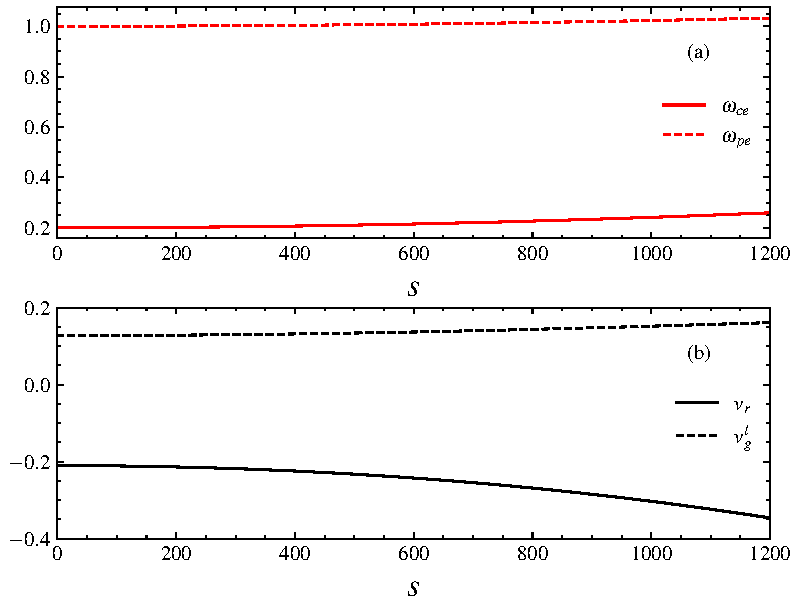
\includegraphics[scale=0.5]{cpc_img/fig_profile.pdf}
        \caption{(a) Background magnetic field and density profile. (b) Characterastic velocity in our simulation.}
        \label{fig.profile}
    \end{figure}
Meanwhile, we show the most unstable wave frequency applied in the simulation for the determination of initial reference frame. According to the choosen parameter in Tab. (\ref{tab.parameters}) and the definition of growth rate  $\gamma_l$ at the equator
\begin{equation}
\begin{aligned}
    \gamma_l(s) & =\frac{\sqrt{2 \pi} \omega_{c e} v_g \omega_{h 0}^2}{4 k_l^2 v_{t h \| 0}} e^{-\frac{\left(\omega_l-\omega_{c e}\right)^2}{2 k_l^2 v_{t h \| 0}}}
    \cdot \left((1+\beta) \frac{T_{\perp 0}}{T_{\| 0}} \frac{\omega_{c e 0}-\omega_l}{\omega_{c e 0}}-1\right)
    \end{aligned}
\end{equation}
The most unstable frequency is $\omega_l = 0.061$ and the corresponding growth rate is $\gamma_l \simeq 3.24\times 10^{-4}$, as shown by a scan of the parameter given in Fig.~\ref{fig.para}.
\begin{figure}[htbp]
    \centering
    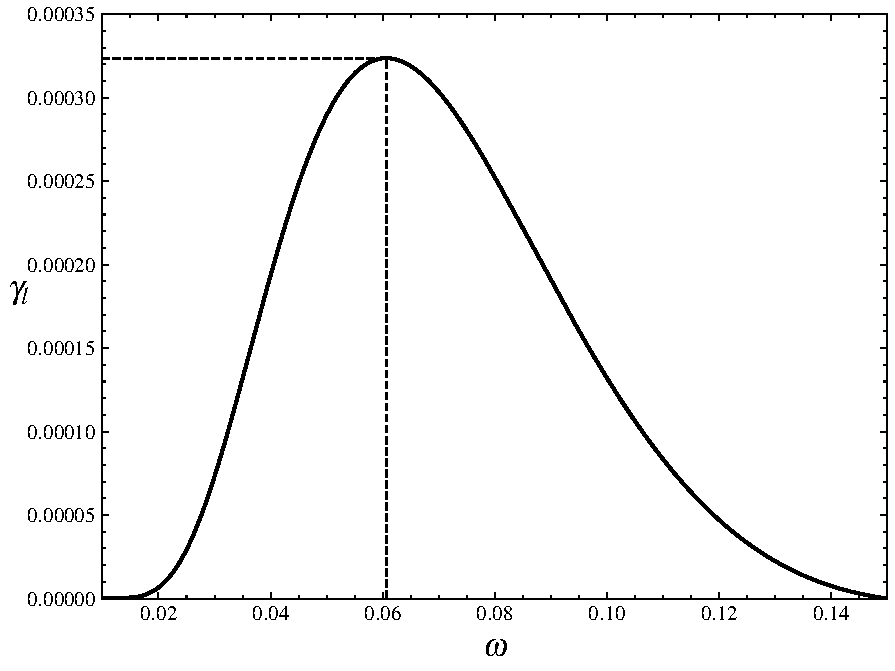
\includegraphics[scale=0.5]{cpc_img/fig_gamma1d.pdf}
    \caption{Linear growth rate $\gamma$ with respect to $\omega$ in the chosen parameter. The initial frequency of the wave is obtained from the most unstable frequency indicated by the vertical black line.}
    \label{fig.para}
\end{figure}

Benefiting from the scale-separated numerical scheme we set the number of grids for wave solver to 1001, which is the same as the sampling points in $s$. 
We apply a delta function in $\mathcal{J}$ dimension, thus only one sampling point is used for $\mathcal{J}$.
For non-delta distribution, tens of samplings points are sufficient for $\mathcal{J}$ sampling. 
As to the $\xi,\Omega$ domain, the Eulerian grids are $31 \times 401$ for $\xi \in [0,2\pi]$ and $\Omega \in [-0.1,0.1]$.

The wave is solved on one dimensional space, thus the workload is relatively small, so as the Lagrangian solver.
The bottle neck is in the Eulerian solver, since it is two dimensional space and hunders of iterations are calculated for one Lagrangian time step for all makers.
However, the computational cost is affordable compared to the conventional PIC simulation, where the sampling points are at least several orders of magnitudes  greater than our method. 
Thus several billions of particles are need in their simulation \cite{nogi2022,katoh2016}.

\subsection{Benchmarks results}
%Here we present several cases to show the feature of our simulation.
%We first present the propagation and growth of the wave by showing four time snapshots of wave complex components in figure~\ref{fig.amp}.
%In the beginning of the simulation, the whistler-mode wave is set at noise level, and the energetic electron anisotropy results in the linear whistler wave instability, and cause the exponential growth of the wave amplitude, indicated in Fig.~\ref{fig.amp}(a). While in Fig.~\ref{fig.amp}(b)-(c), after the wave amplitude reached sufficient level, nonlinear resonant trapping occurs, and the chorus wave is initially triggered near the equator by the resonant electrons moving from the right to the left. The wave is propagating in the opposite direction to the resonant particles, chirping and amplifying continuously in this stage.
%\begin{figure}[htbp]
%    \centering
%    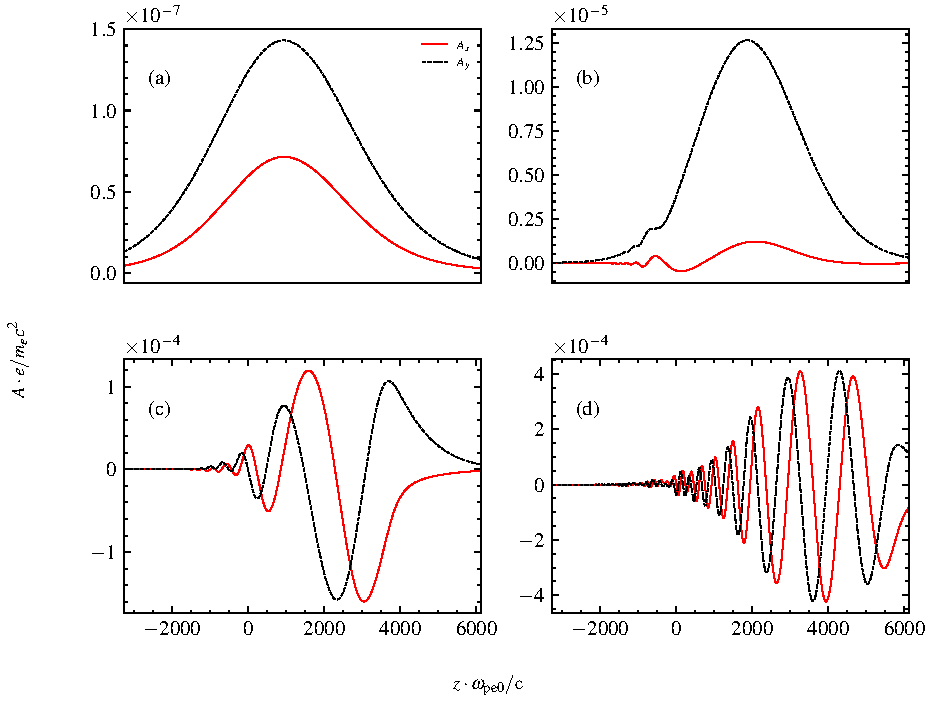
\includegraphics[scale=0.5]{cpc_img/fig_amp.pdf}
%    \caption{Time snapshots of wave complex amplitude. The red and black curves represent the real and imaginary components of the complex vector potential, respectively. Subplots (a)-(d) indicate the wave amplitude at different time.}
%    \label{fig.amp}
%\end{figure}
%In the meantime, one can see that the location of the maximal wave amplitude changes sightly in different time stage, which indicates that the linear whistler wave is propagating to the right pole. 
The linear physics are verified quantitatively in Fig.~\ref{fig.linear}, where we calculate the growth rate and the velocity of the maximum wave amplitude location before the nonlinearity take over. 
For the propagating wave, the trajectory for the wave packet is caluclated from the group velocity integral
\begin{equation}
    s(t) = s(0) + \int_0^{t} v_g(s(\tau)) \mathrm{d} \tau~.
\end{equation}
Here we trace the movement of the maximum amplitude point. Its propagation is in accord with the linear group velocity, as shown in Fig. \ref{fig.linear}(a). 
For the wave peak, it indeed propagates in the linear group velocity during the linear stage.
Moreover, we estimate the amplitude growth of the wave peak along its propagation path, the growth rate is given by \cite{nogi2022}
\begin{equation}\label{eq.gm_ver}
        \Gamma = \frac{1}{t_1-t_0}\log\frac{|a(s_1,t_1)|}{|a(s_0,t_0)|}~,
\end{equation}
where $s_0,t_0$, $s_1,t_1$ are along the prppagation path.
The growth of the amplitude along the propatation path is shown in Fig. \ref{fig.linear}(b). The corresponding growth rate from equation (\ref{eq.gm_ver}) is $\Gamma_0 \simeq 3.21\times10^{-4}$, agrees well with the theoretic linear growth rate shown in Fig. \ref{fig.para}.
The results show the correctness of our simulation at linear stage.
\begin{figure}[htbp]
    \centering
    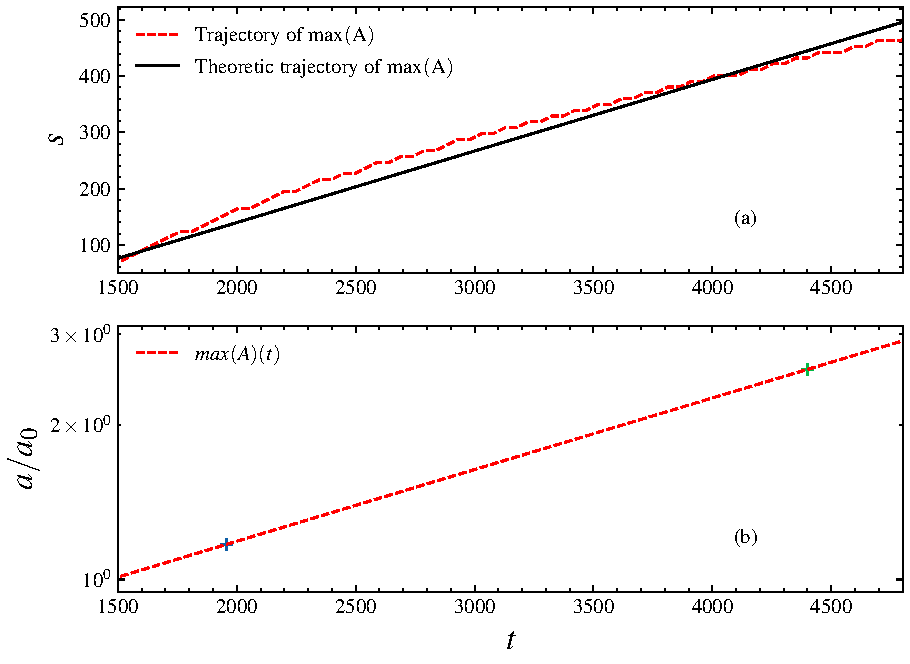
\includegraphics[scale=0.5]{cpc_img/fig_linear.pdf}
    \caption{Figure (a) is the propagation velocity of the linear wave packet with the maximum amplitude. Figure (b) denotes the growth of the wave peak amplitude with time along wave propagation path. The green cross marks the point used to caluclate the growth rate.}
    \label{fig.linear}
\end{figure}

%Other than the linear physics seen from Fig.~\ref{fig.amp}(a), we can see that the generation, amplification, and propagation of the nonlinear chorus wave in Fig.~\ref{fig.amp}(b-d). The phase difference between the $a_x$ and $a_y$ components is $\pi/2$ for the nonlinear chorus wave, which is the characterastic of right hand polarized wave. The wave tail becomes more oscillatory, and eventually out of phase near the equator at the end. The reason is that the numerical breakdown of the periodic boundary condition in our simulation. Besides, the most important feature, i.e., the frequency sweeping in this case is shown in figure~\ref{fig.chirping}~(a). The frequency of chorus in our simulation is calculated using the definition of eikonal function, i.e. $\omega = \partial \phi/\partial t$. In addition, we apply empirical mode decomposition (EMD) on the original data to separate the main component and high order frequency oscillation due to finite bandwidth of chorus.
%
%\begin{figure}[htbp]
%    \centering
%    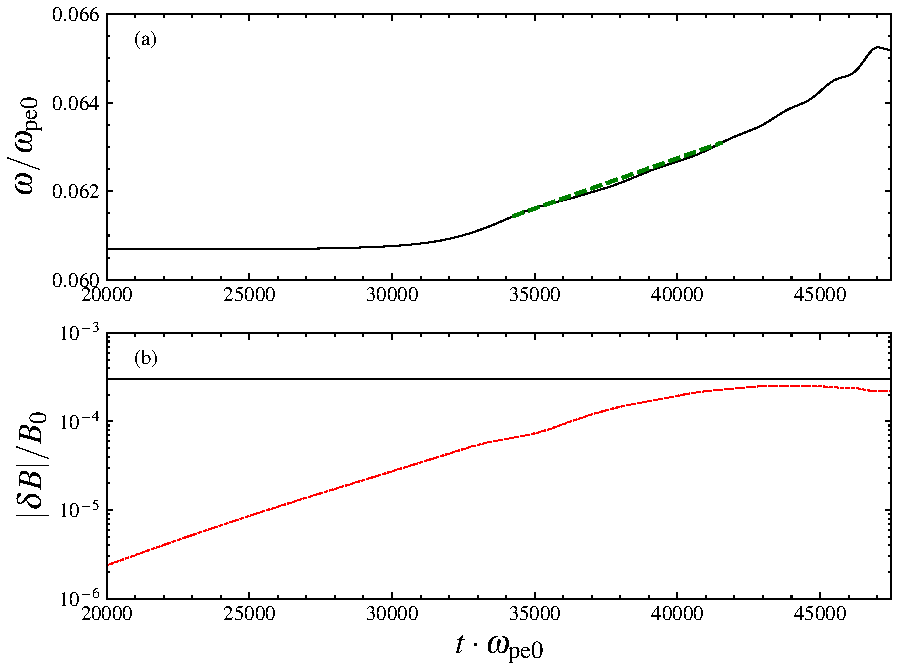
\includegraphics[scale=0.5]{cpc_img/fig_nonlinear.pdf}
%    \caption{The evolution of the wave frequency and amplitude, where (a) is the frequency chirping and (b) denotes the amplitude growth. The frequency evolution at position $s = 531$ is present. Wave amplitude is given in magnetic field induction $\delta B/B_0$, where $B_0$ is the background magnetic field at the magnetic equator.}
%    \label{fig.chirping}
%\end{figure}
%
%In the liner stage, the wave frequency remains constant, and at around $t = 30000$, wave frequency is increasing from the most unstable frequency $w_l = 0.061$, and chirped to around $0.065$ in 12500 electron oscillation periods. The corresponding chirping rate is about $2.38~\mathrm{kHz/s}$, agrees well with the observation. The wave growth shown in Fig.~\ref{fig.chirping}~(b) have the same tendency. At the linear stage, the wave is exponential growing, and begin to saturate at nonlinear stage, the saturation level is around $2.5 \times 10^{-4} B_0$, also in well agree with the observation and other numerical simulations.


In the nonlinear stage, the trapped electrons forms a hole in the phase space $\xi-\Omega$. The phase space hole contributes the nonlinear current that triggers the nonlinear frequency chiping chorus wave \cite{omura2008}. 
The shape of the hole, i.e., its boundary, can be analytically given by 
\begin{equation}\label{eq.Omega_b}
    \Omega(\xi) = \pm \frac{\omega_b}{k^2} \sqrt{2 (e_{spx}-\cos \xi - \alpha \xi)}
\end{equation}
where $e_{spx}$ is the particle energy on the separatrix, $k$ is the wave number and $\omega_b\equiv \sqrt{k^2 v_\perp a}$ is the trapped particle bounce frequency.
The parameter is the inhomogeneity ratio \cite{omura2008,tao2020}
\begin{equation}\label{eq.alp}
    \alpha \equiv \frac{1}{\omega_{b}^2}\left[\left(1 - 2\frac{v_r}{v_g}\right)\frac{\partial \omega}{\partial t}  -v_r^2 \frac{\partial k}{\partial s}+ \frac{\mathrm{\partial} \omega_{ce}}{\mathrm{\partial} s}\frac{k_i}{m_e}\mathcal{J}\right].
\end{equation}
In Fig.~\ref{fig.hole}, we show a typical electron phase-space hole at a given $s$ the late nonlinear stage. We calculated the corresponding $k \simeq 0.649$, $\omega_b \simeq 0.007$, $\alpha \simeq 0.08$ at the location from the simulation data, and we depicted the boundary of the hole from equation (\ref{eq.Omega_b}). The shape of the hole well matches with the theoretic results.

\begin{figure}[htbp]
    \centering
    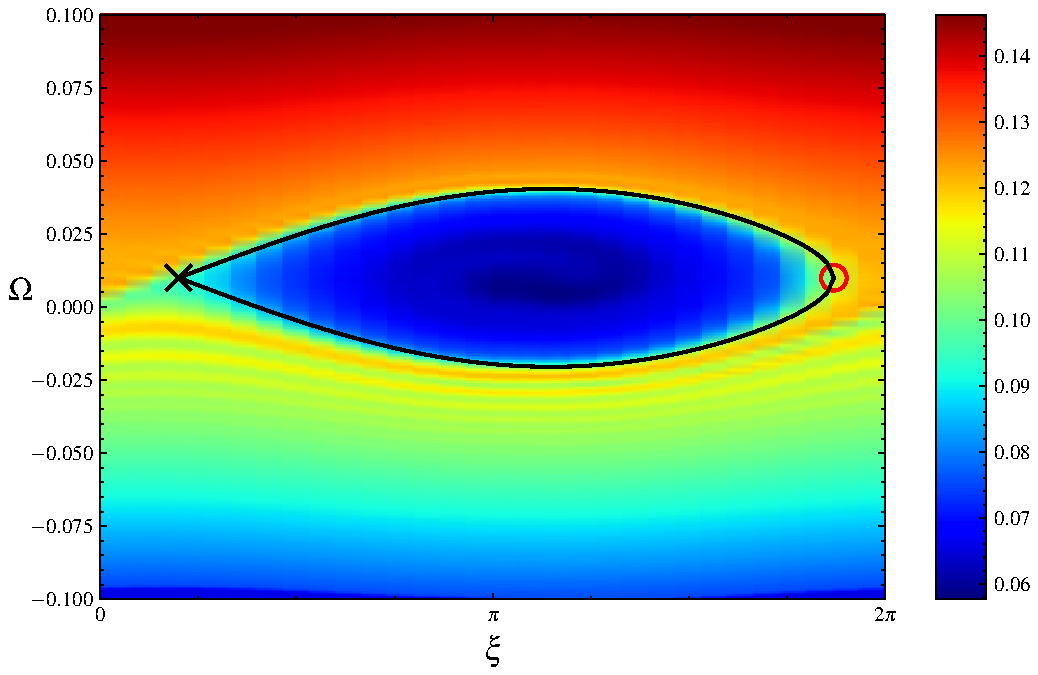
\includegraphics[scale=0.5]{cpc_img/fig_hole.pdf}
    \caption{Phase-space hole formed by trapped electrons in the wave field. The size and location of the hole, i.e., the X, C points, and the boundary, are determined from the nonlinear theory.}
    \label{fig.hole}
\end{figure}


